\documentclass{beamer}

\mode<presentation> {
\usetheme{AnnArbor}
}

\usepackage{graphicx}
\graphicspath{{./figures/}}
\usepackage{caption}
\usepackage{subcaption}
\usepackage{hyperref}
\hypersetup{colorlinks=true}
\usepackage{amsmath}
\usepackage{biblatex}
\addbibresource{bibliography.bib}

\title[Univariate Extreme Value Theory]{Univariate Extreme Value Theory}

\author{Victor Verma}
\institute[]
{
Prof. Yang Chen's Reading Group \\
Department of Statistics \\
University of Michigan
}
\date[1/26/23]{1/26/23} 

\begin{document}

\begin{frame}
    \titlepage
\end{frame}

\begin{frame}{Today's Reading}
    \begin{itemize}
        \item Chapter 3 of \textit{Modelling Extremal Events} by Embrechts, Kl\"{u}ppelberg, and Mikosch (\cite{embrechts_et_al_1997})
    \end{itemize}
\end{frame}

\begin{frame}{Outline}
    \tableofcontents
\end{frame}

\begin{frame}{An Example Problem}
    \begin{figure}
        \centering
        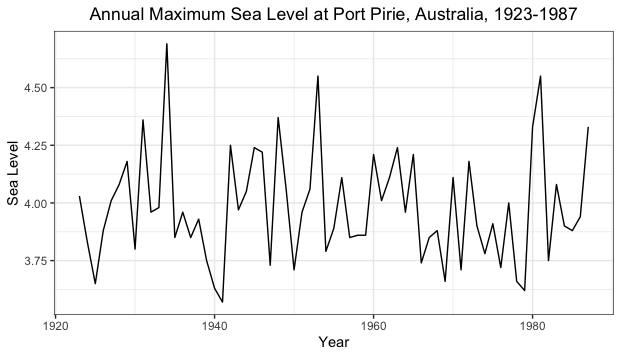
\includegraphics[scale=0.5]{max_sea_levels.png}
        \caption{Annual maximum sea levels at Port Pirie, Australia, 1923-1987.}
        \label{fig:max_sea_levels}
    \end{figure}    
\end{frame}

\begin{frame}{An Example Problem}
    Some questions:
    \begin{itemize}
        \item What sea level is observed once every 100 years? every 1,000 years?
    \end{itemize}

    A necessary assumption:
    \begin{itemize}
        \item Current climactic conditions will persist
    \end{itemize}

    \bigskip
    
    Some terminology:
    \begin{itemize}
        \item An event with probability $p$ has \textbf{return period} $1 / p$
        \item The \textbf{return level} with return period $1 / p$ is the upper $p$th quantile of the distribution
    \end{itemize}
    The annual maximum sea level observed once every 100 years is the return level with return period $1 / 100 = 0.01$.
\end{frame}

\begin{frame}{An Example Problem}
    Some notation:
    \begin{itemize}
        \item Let $X \sim F$ be the sea level on a day.
        \item Let $M_n = \max_{i = 1, \ldots, n} X_i$ be the maximum over a period of $n$ days.
    \end{itemize}
    The return level with return period 0.01 is $m_{0.01}$, the upper 0.01 quantile of $F^{365}$, the df of $M_{365}$.

    \bigskip

    How to estimate $m_{0.01}$?
\end{frame}

\begin{frame}{An Example Problem}
    One idea:
    \begin{itemize}
        \item Approximate $F$ by $\hat{F}$, then approximate $F^{365}$ by $\hat{F}^{365}$.
        \begin{itemize}
            \item The error in $\hat{F}$ will get compounded.
        \end{itemize}
    \end{itemize}

    Another idea:
    \begin{itemize}
        \item Directly approximate $F^{365}$ using the the asymptotic behavior of $M_n$.
        \item If $F^n \xrightarrow{d} G$ for some df G, then $F^n \approx G$ for large $n$, like 365.
    \end{itemize}
\end{frame}

\begin{frame}{The Block Maximum Approach}
    $M_n$ is a \textbf{block maximum}. The block maximum approach to extreme value analysis:
    \begin{itemize}
        \item Divide data $X_1, X_2, X_3, \ldots \overset{\text{iid}} F$ into blocks of size $n$
        \item Find a $G$ such that $F^n \xrightarrow{d} G$.
        \item Use $G$ to approximate $F^n$ for $n$ of interest
    \end{itemize}
\end{frame}

\begin{frame}{The Block Maximum Approach, First Attempt}
    The \textbf{right endpoint} of $F$ is
    \begin{align*}
    x_F &= \sup\{x \in \mathbb{R} : F(x) < 1\} \\
    &= \inf\{x \in \mathbb{R} : F(x) = 1\}
    \end{align*}
    If $x_F < \infty$, then $M_n \xrightarrow{d} x_F$. $F_{x_F}$ is a bad approximation to $F^n$ because it is \textbf{degenerate}.

    \bigskip

    What to do?
\end{frame}

\begin{frame}{The Block Maximum Approach, Second Attempt}
    In the CLT, $S_n = \sum_{i = 1}^n X_i$ is \textbf{normalized}:
    \[
    \frac{\sqrt{n}}{\sigma}(S_n - \mu) \xrightarrow{d} N(0, 1)
    \]
    Idea: Normalize $M_n$ - consider $c_n^{-1}(M_n - d_n)$ as $n \to \infty$. If $c_n^{-1}(M_n - d_n) \xrightarrow{d} G$ and $G$ is nondegenerate, then for large $n$,
    \begin{align*}
        P(M_n \le x) &= P(c_n^{-1}(M_n - d_n) \le c_n^{-1}(x - d_n)) \\
        &\approx G(c_n^{-1}(x - d_n)).
    \end{align*}
\end{frame}

\section{References}

\begin{frame}[allowframebreaks]{References}
    \nocite{*}
    \printbibliography
\end{frame}

\end{document} 